% Created by tikzDevice version 0.10.1 on 2016-09-01 14:06:06
% !TEX encoding = UTF-8 Unicode
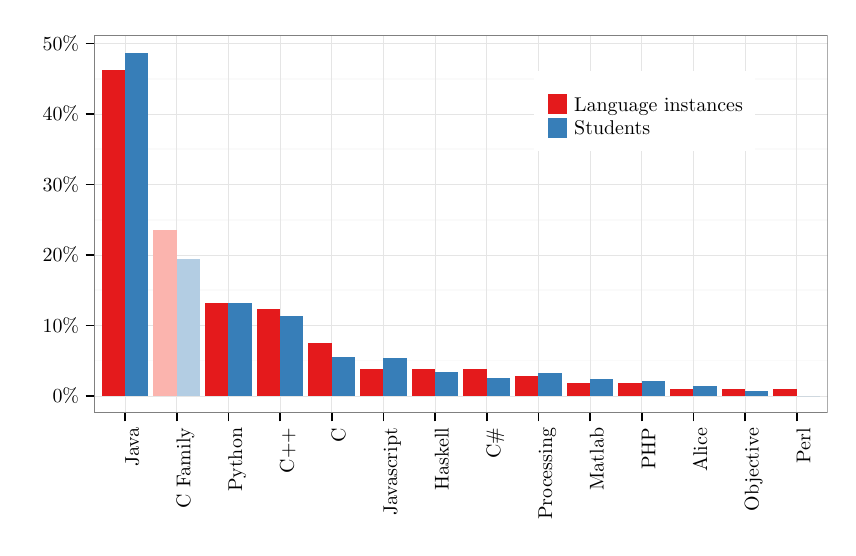
\begin{tikzpicture}[x=1pt,y=1pt]
\definecolor{fillColor}{RGB}{255,255,255}
\path[use as bounding box,fill=fillColor,fill opacity=0.00] (0,0) rectangle (289.08,180.67);
\begin{scope}
\path[clip] (  0.00,  0.00) rectangle (289.08,180.67);
\definecolor{drawColor}{RGB}{255,255,255}
\definecolor{fillColor}{RGB}{255,255,255}

\path[draw=drawColor,line width= 0.6pt,line join=round,line cap=round,fill=fillColor] (  0.00,  0.00) rectangle (289.08,180.68);
\end{scope}
\begin{scope}
\path[clip] ( 23.98, 41.44) rectangle (289.08,177.83);
\definecolor{fillColor}{RGB}{255,255,255}

\path[fill=fillColor] ( 23.98, 41.44) rectangle (289.08,177.83);
\definecolor{drawColor}{gray}{0.98}

\path[draw=drawColor,line width= 0.6pt,line join=round] ( 23.98, 60.37) --
	(289.08, 60.37);

\path[draw=drawColor,line width= 0.6pt,line join=round] ( 23.98, 85.83) --
	(289.08, 85.83);

\path[draw=drawColor,line width= 0.6pt,line join=round] ( 23.98,111.29) --
	(289.08,111.29);

\path[draw=drawColor,line width= 0.6pt,line join=round] ( 23.98,136.76) --
	(289.08,136.76);

\path[draw=drawColor,line width= 0.6pt,line join=round] ( 23.98,162.22) --
	(289.08,162.22);
\definecolor{drawColor}{gray}{0.90}

\path[draw=drawColor,line width= 0.2pt,line join=round] ( 23.98, 47.64) --
	(289.08, 47.64);

\path[draw=drawColor,line width= 0.2pt,line join=round] ( 23.98, 73.10) --
	(289.08, 73.10);

\path[draw=drawColor,line width= 0.2pt,line join=round] ( 23.98, 98.56) --
	(289.08, 98.56);

\path[draw=drawColor,line width= 0.2pt,line join=round] ( 23.98,124.03) --
	(289.08,124.03);

\path[draw=drawColor,line width= 0.2pt,line join=round] ( 23.98,149.49) --
	(289.08,149.49);

\path[draw=drawColor,line width= 0.2pt,line join=round] ( 23.98,174.95) --
	(289.08,174.95);

\path[draw=drawColor,line width= 0.2pt,line join=round] ( 35.18, 41.44) --
	( 35.18,177.83);

\path[draw=drawColor,line width= 0.2pt,line join=round] ( 53.85, 41.44) --
	( 53.85,177.83);

\path[draw=drawColor,line width= 0.2pt,line join=round] ( 72.52, 41.44) --
	( 72.52,177.83);

\path[draw=drawColor,line width= 0.2pt,line join=round] ( 91.19, 41.44) --
	( 91.19,177.83);

\path[draw=drawColor,line width= 0.2pt,line join=round] (109.86, 41.44) --
	(109.86,177.83);

\path[draw=drawColor,line width= 0.2pt,line join=round] (128.53, 41.44) --
	(128.53,177.83);

\path[draw=drawColor,line width= 0.2pt,line join=round] (147.20, 41.44) --
	(147.20,177.83);

\path[draw=drawColor,line width= 0.2pt,line join=round] (165.86, 41.44) --
	(165.86,177.83);

\path[draw=drawColor,line width= 0.2pt,line join=round] (184.53, 41.44) --
	(184.53,177.83);

\path[draw=drawColor,line width= 0.2pt,line join=round] (203.20, 41.44) --
	(203.20,177.83);

\path[draw=drawColor,line width= 0.2pt,line join=round] (221.87, 41.44) --
	(221.87,177.83);

\path[draw=drawColor,line width= 0.2pt,line join=round] (240.54, 41.44) --
	(240.54,177.83);

\path[draw=drawColor,line width= 0.2pt,line join=round] (259.21, 41.44) --
	(259.21,177.83);

\path[draw=drawColor,line width= 0.2pt,line join=round] (277.88, 41.44) --
	(277.88,177.83);
\definecolor{fillColor}{RGB}{228,26,28}

\path[fill=fillColor] ( 26.78, 47.64) rectangle ( 35.18,165.34);
\definecolor{fillColor}{RGB}{55,126,184}

\path[fill=fillColor] ( 35.18, 47.64) rectangle ( 43.58,171.63);
\definecolor{fillColor}{RGB}{251,180,174}

\path[fill=fillColor] ( 45.45, 47.64) rectangle ( 53.85,107.69);
\definecolor{fillColor}{RGB}{179,205,227}

\path[fill=fillColor] ( 53.85, 47.64) rectangle ( 62.25, 97.19);
\definecolor{fillColor}{RGB}{228,26,28}

\path[fill=fillColor] ( 64.12, 47.64) rectangle ( 72.52, 81.27);
\definecolor{fillColor}{RGB}{55,126,184}

\path[fill=fillColor] ( 72.52, 47.64) rectangle ( 80.92, 81.34);
\definecolor{fillColor}{RGB}{228,26,28}

\path[fill=fillColor] ( 82.79, 47.64) rectangle ( 91.19, 78.86);
\definecolor{fillColor}{RGB}{55,126,184}

\path[fill=fillColor] ( 91.19, 47.64) rectangle ( 99.59, 76.55);
\definecolor{fillColor}{RGB}{228,26,28}

\path[fill=fillColor] (101.46, 47.64) rectangle (109.86, 66.85);
\definecolor{fillColor}{RGB}{55,126,184}

\path[fill=fillColor] (109.86, 47.64) rectangle (118.26, 61.82);
\definecolor{fillColor}{RGB}{228,26,28}

\path[fill=fillColor] (120.13, 47.64) rectangle (128.53, 57.25);
\definecolor{fillColor}{RGB}{55,126,184}

\path[fill=fillColor] (128.53, 47.64) rectangle (136.93, 61.18);
\definecolor{fillColor}{RGB}{228,26,28}

\path[fill=fillColor] (138.79, 47.64) rectangle (147.20, 57.25);
\definecolor{fillColor}{RGB}{55,126,184}

\path[fill=fillColor] (147.20, 47.64) rectangle (155.60, 56.40);
\definecolor{fillColor}{RGB}{228,26,28}

\path[fill=fillColor] (157.46, 47.64) rectangle (165.86, 57.25);
\definecolor{fillColor}{RGB}{55,126,184}

\path[fill=fillColor] (165.86, 47.64) rectangle (174.27, 54.09);
\definecolor{fillColor}{RGB}{228,26,28}

\path[fill=fillColor] (176.13, 47.64) rectangle (184.53, 54.84);
\definecolor{fillColor}{RGB}{55,126,184}

\path[fill=fillColor] (184.53, 47.64) rectangle (192.93, 55.83);
\definecolor{fillColor}{RGB}{228,26,28}

\path[fill=fillColor] (194.80, 47.64) rectangle (203.20, 52.44);
\definecolor{fillColor}{RGB}{55,126,184}

\path[fill=fillColor] (203.20, 47.64) rectangle (211.60, 53.77);
\definecolor{fillColor}{RGB}{228,26,28}

\path[fill=fillColor] (213.47, 47.64) rectangle (221.87, 52.44);
\definecolor{fillColor}{RGB}{55,126,184}

\path[fill=fillColor] (221.87, 47.64) rectangle (230.27, 53.05);
\definecolor{fillColor}{RGB}{228,26,28}

\path[fill=fillColor] (232.14, 47.64) rectangle (240.54, 50.04);
\definecolor{fillColor}{RGB}{55,126,184}

\path[fill=fillColor] (240.54, 47.64) rectangle (248.94, 51.11);
\definecolor{fillColor}{RGB}{228,26,28}

\path[fill=fillColor] (250.81, 47.64) rectangle (259.21, 50.04);
\definecolor{fillColor}{RGB}{55,126,184}

\path[fill=fillColor] (259.21, 47.64) rectangle (267.61, 49.49);
\definecolor{fillColor}{RGB}{228,26,28}

\path[fill=fillColor] (269.48, 47.64) rectangle (277.88, 50.04);
\definecolor{fillColor}{RGB}{55,126,184}

\path[fill=fillColor] (277.88, 47.64) rectangle (286.28, 47.64);
\definecolor{drawColor}{gray}{0.50}

\path[draw=drawColor,line width= 0.6pt,line join=round,line cap=round] ( 23.98, 41.44) rectangle (289.08,177.83);
\end{scope}
\begin{scope}
\path[clip] (  0.00,  0.00) rectangle (289.08,180.67);
\definecolor{drawColor}{RGB}{0,0,0}

\node[text=drawColor,anchor=base east,inner sep=0pt, outer sep=0pt, scale=  0.72] at ( 18.58, 45.16) {0\%};

\node[text=drawColor,anchor=base east,inner sep=0pt, outer sep=0pt, scale=  0.72] at ( 18.58, 70.62) {10\%};

\node[text=drawColor,anchor=base east,inner sep=0pt, outer sep=0pt, scale=  0.72] at ( 18.58, 96.08) {20\%};

\node[text=drawColor,anchor=base east,inner sep=0pt, outer sep=0pt, scale=  0.72] at ( 18.58,121.55) {30\%};

\node[text=drawColor,anchor=base east,inner sep=0pt, outer sep=0pt, scale=  0.72] at ( 18.58,147.01) {40\%};

\node[text=drawColor,anchor=base east,inner sep=0pt, outer sep=0pt, scale=  0.72] at ( 18.58,172.47) {50\%};
\end{scope}
\begin{scope}
\path[clip] (  0.00,  0.00) rectangle (289.08,180.67);
\definecolor{drawColor}{RGB}{0,0,0}

\path[draw=drawColor,line width= 0.6pt,line join=round] ( 20.98, 47.64) --
	( 23.98, 47.64);

\path[draw=drawColor,line width= 0.6pt,line join=round] ( 20.98, 73.10) --
	( 23.98, 73.10);

\path[draw=drawColor,line width= 0.6pt,line join=round] ( 20.98, 98.56) --
	( 23.98, 98.56);

\path[draw=drawColor,line width= 0.6pt,line join=round] ( 20.98,124.03) --
	( 23.98,124.03);

\path[draw=drawColor,line width= 0.6pt,line join=round] ( 20.98,149.49) --
	( 23.98,149.49);

\path[draw=drawColor,line width= 0.6pt,line join=round] ( 20.98,174.95) --
	( 23.98,174.95);
\end{scope}
\begin{scope}
\path[clip] (  0.00,  0.00) rectangle (289.08,180.67);
\definecolor{drawColor}{RGB}{0,0,0}

\path[draw=drawColor,line width= 0.6pt,line join=round] ( 35.18, 38.44) --
	( 35.18, 41.44);

\path[draw=drawColor,line width= 0.6pt,line join=round] ( 53.85, 38.44) --
	( 53.85, 41.44);

\path[draw=drawColor,line width= 0.6pt,line join=round] ( 72.52, 38.44) --
	( 72.52, 41.44);

\path[draw=drawColor,line width= 0.6pt,line join=round] ( 91.19, 38.44) --
	( 91.19, 41.44);

\path[draw=drawColor,line width= 0.6pt,line join=round] (109.86, 38.44) --
	(109.86, 41.44);

\path[draw=drawColor,line width= 0.6pt,line join=round] (128.53, 38.44) --
	(128.53, 41.44);

\path[draw=drawColor,line width= 0.6pt,line join=round] (147.20, 38.44) --
	(147.20, 41.44);

\path[draw=drawColor,line width= 0.6pt,line join=round] (165.86, 38.44) --
	(165.86, 41.44);

\path[draw=drawColor,line width= 0.6pt,line join=round] (184.53, 38.44) --
	(184.53, 41.44);

\path[draw=drawColor,line width= 0.6pt,line join=round] (203.20, 38.44) --
	(203.20, 41.44);

\path[draw=drawColor,line width= 0.6pt,line join=round] (221.87, 38.44) --
	(221.87, 41.44);

\path[draw=drawColor,line width= 0.6pt,line join=round] (240.54, 38.44) --
	(240.54, 41.44);

\path[draw=drawColor,line width= 0.6pt,line join=round] (259.21, 38.44) --
	(259.21, 41.44);

\path[draw=drawColor,line width= 0.6pt,line join=round] (277.88, 38.44) --
	(277.88, 41.44);
\end{scope}
\begin{scope}
\path[clip] (  0.00,  0.00) rectangle (289.08,180.67);
\definecolor{drawColor}{RGB}{0,0,0}

\node[text=drawColor,rotate= 90.00,anchor=base east,inner sep=0pt, outer sep=0pt, scale=  0.72] at ( 40.14, 36.04) {Java};

\node[text=drawColor,rotate= 90.00,anchor=base east,inner sep=0pt, outer sep=0pt, scale=  0.72] at ( 58.81, 36.04) {C Family};

\node[text=drawColor,rotate= 90.00,anchor=base east,inner sep=0pt, outer sep=0pt, scale=  0.72] at ( 77.48, 36.04) {Python};

\node[text=drawColor,rotate= 90.00,anchor=base east,inner sep=0pt, outer sep=0pt, scale=  0.72] at ( 96.15, 36.04) {C++};

\node[text=drawColor,rotate= 90.00,anchor=base east,inner sep=0pt, outer sep=0pt, scale=  0.72] at (114.82, 36.04) {C};

\node[text=drawColor,rotate= 90.00,anchor=base east,inner sep=0pt, outer sep=0pt, scale=  0.72] at (133.48, 36.04) {Javascript};

\node[text=drawColor,rotate= 90.00,anchor=base east,inner sep=0pt, outer sep=0pt, scale=  0.72] at (152.15, 36.04) {Haskell};

\node[text=drawColor,rotate= 90.00,anchor=base east,inner sep=0pt, outer sep=0pt, scale=  0.72] at (170.82, 36.04) {C\#};

\node[text=drawColor,rotate= 90.00,anchor=base east,inner sep=0pt, outer sep=0pt, scale=  0.72] at (189.49, 36.04) {Processing};

\node[text=drawColor,rotate= 90.00,anchor=base east,inner sep=0pt, outer sep=0pt, scale=  0.72] at (208.16, 36.04) {Matlab};

\node[text=drawColor,rotate= 90.00,anchor=base east,inner sep=0pt, outer sep=0pt, scale=  0.72] at (226.83, 36.04) {PHP};

\node[text=drawColor,rotate= 90.00,anchor=base east,inner sep=0pt, outer sep=0pt, scale=  0.72] at (245.50, 36.04) {Alice};

\node[text=drawColor,rotate= 90.00,anchor=base east,inner sep=0pt, outer sep=0pt, scale=  0.72] at (264.17, 36.04) {Objective};

\node[text=drawColor,rotate= 90.00,anchor=base east,inner sep=0pt, outer sep=0pt, scale=  0.72] at (282.84, 36.04) {Perl};
\end{scope}
\begin{scope}
\path[clip] (  0.00,  0.00) rectangle (289.08,180.67);
\definecolor{fillColor}{RGB}{255,255,255}

\path[fill=fillColor] (182.88,135.94) rectangle (262.73,165.16);
\end{scope}
\begin{scope}
\path[clip] (  0.00,  0.00) rectangle (289.08,180.67);
\definecolor{fillColor}{RGB}{228,26,28}

\path[fill=fillColor] (187.86,149.46) rectangle (194.98,156.57);
\end{scope}
\begin{scope}
\path[clip] (  0.00,  0.00) rectangle (289.08,180.67);
\definecolor{fillColor}{RGB}{55,126,184}

\path[fill=fillColor] (187.86,140.92) rectangle (194.98,148.03);
\end{scope}
\begin{scope}
\path[clip] (  0.00,  0.00) rectangle (289.08,180.67);
\definecolor{drawColor}{RGB}{0,0,0}

\node[text=drawColor,anchor=base west,inner sep=0pt, outer sep=0pt, scale=  0.72] at (197.49,150.53) {Language instances};
\end{scope}
\begin{scope}
\path[clip] (  0.00,  0.00) rectangle (289.08,180.67);
\definecolor{drawColor}{RGB}{0,0,0}

\node[text=drawColor,anchor=base west,inner sep=0pt, outer sep=0pt, scale=  0.72] at (197.49,142.00) {Students};
\end{scope}
\end{tikzpicture}
